The \verb=Analysis= module reads the ADC signal and puts out information on how to draw two bars (one for each speaker) that reflect the power of said signal. Since we want bars for before and after modulation, we'll use two instances of the same module. 

The required inputs include a left or right selection signal to specify which stereo channel we are about to analyse, two 16-bit signed ADC/DAC signals (left and right), and \verb=vsync= lined from \verb+VGA_Driver+. There are two 8-bit unsigned output signals (once again, one left, one right). They determine the height of the bar which the \verb=VGA_Driver= should render.

The incoming signals are low pass filtered with a saturation time of approximately 100 ms (4096 sample cycles) as seen in figure \ref{fig:lowpass}, resulting in a measurement of the signal's power. 

\begin{figure}[h]
\centering
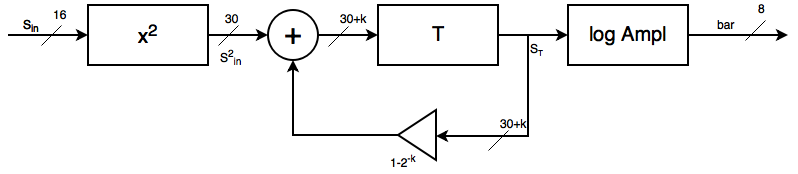
\includegraphics[width=16cm]{lowpass}
\caption{The low pass filter. $k$ is chosen by the approximation $\frac{1}{10}\mathrm{\ s} = 2^k\cdot\frac{1}{48800}\Rightarrow 2^k=4880\approx 2^{12}\Rightarrow k = 12 $}
\label{fig:lowpass}
\end{figure}

\verb=log_Pow= takes the logarithm of the low pass filtered signal. It provides module outputs proportional to the result, updating only in sync with \verb+vsync+. The \verb+bar+ signals are lined to \verb+VGA_Driver+ as definitive information about how the power bars should render on screen.

$S_T$ in the picture above is initially stored in a register, while setting a decrementing counter to the width of the signal. Every clock cycle, the MSB is checked for a '1' in conjunction with a left shift of the register's bits. Once a '1' is found, the counter gives us the logarithm - essentially, the index of the most significant '1'. We then concatenate the value of our counter with the following two MSBs remaining in the shifted register. This result represents the pixel height of the specific bar to be rendered. \verb=lrsel= determines which stereo channel should be read and thus which bar height should be written to at any given time.

As a closing tidbit, \verb=counter & shiftreg(MSB downto MSB-1)= can, read as unsigned, give a maximum value of 171, since \verb=counter= at most is equal to $\mathtt{S_T}$\verb='length=.
